\documentclass[10pt,conference,compsocconf]{IEEEtran}

\usepackage{hyperref}
\usepackage{graphicx}	% For figure environment

\begin{document}
\title{Earthquake Detection from Seismological Data}

\author{
  Lucien Michaël Iseli, Florian Maxime Charles Ravasi and Jules Eliot Gottraux\\
  \textit{Master of Data Science, EPFL, Switzerland}
}

\maketitle
\section{Introduction}

\section{Dataset Characteristics}
We get our data using the ObsPy [1] library. This library permits to easily access signal over time of seismological sensors. Those sensors record  constantly the activity, or vibration, of the earth at their location. This include seismic waves which are the waves of energy released when a seism occur nearby. This dataset contains a significant amount of noise as it is a completely raw measure. It has the information of the seism and earthquake but this information is aggregated with all the vibration happening near the sensor. The data is thus a time series of amplitude of waves captured by the sensor.

\begin{figure}[h]
  \centering
	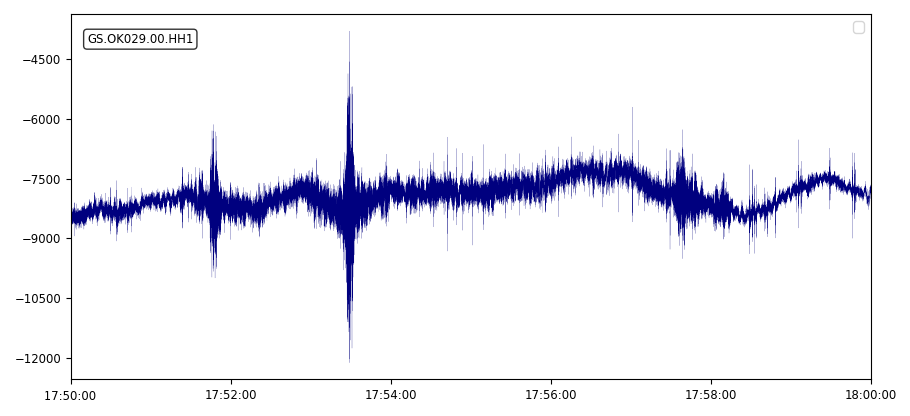
\includegraphics[width=\columnwidth]{../processed-data/10min-example-2018-06-30T17:50.png}
  \caption{10 minute of data example, no earthquake}
	\label{fig:10min-example}
\end{figure}

Those time series are the feature that will be used to do the prediction, for the labels we use a hand-made catalog of earthquake that contains, among other properties, the location, magnitude and time of the earthquake.\newline \newline


Before diving into the machine learning model construction, we have to take care of several difficulties inerrant to the dataset.\newline
First the data collection, after having choosing the location, station and channel from which we want to get the time series we have to download it and store that to a usable format for the next steps. The frequency of the sensors is $100$ data point per second, so the amount of data increase quite quickly. Then, the data has holes in it, the data is missing for some period of time because of casualties or maintenance. Those holes are not regular and unpredictable, so we have to take care of this with caution.

\begin{figure}[h]
  \centering
	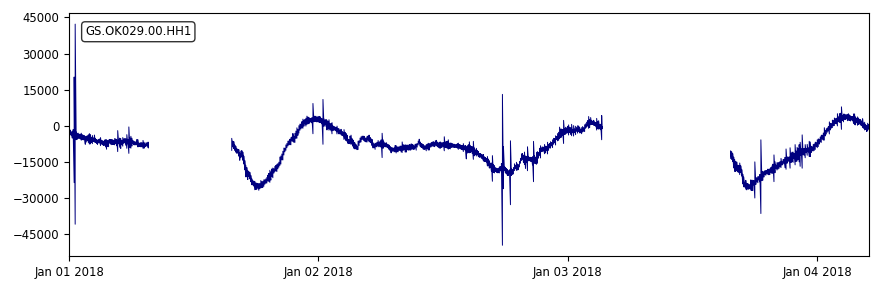
\includegraphics[width=\columnwidth]{../processed-data/hole_example.png}
  \caption{Example of missing values in the dataset}
	\label{fig:10min-example}
\end{figure}

We already discussed the fact that the time series obtained from ObsPy are very noisy, we want to emphasize this and as we will see in examples, some earthquakes and non-earthquakes are undistinguishable for the untrained eye. The catalog is noisy in a sense as well, the time series are parsed by human and thus some earthquakes are missed and as the magnitude decreases the number of missed earthquake increases, becing the majority for small magnitudes. Another difficulty in the catalog is the delay that is induced by the difference of location between the detection of the earthquake and the location of our station. All the catalog have to be calibrated to ensure that the time of earthquake corresponds to a peak in our time series.

\section{Data pre-processing}
Develop the pre-processing steps introduced in last section:
- Fill holes in data\\
- Fix delay of catalog\\

\section{Labeling of the Data}
As the dataset live in a continuous space, we have to discretize it. We have to choose time windows that will be classified as earthquake or not earthquake. The choice of the time is crucial and it is hard to predict what would be a good choice. Also, that give rise to a fundamental question for the creation of the labels: when does an earthquake ends? It is possible, in fact rather probable depending on the length of the discretization process, that an earthquake spans over multiple time window thus knowing the duration of the earthquake would permit to overcome this issue. This is important, because not being able to accurately and correctly label our data will of course be disastrous for the machine learning model. Unfortunately, the duration of an earthquake is an open question in geology, the only option simple enough is to label as earthquake only the window that contains the moment of an earthquake.

\begin{figure}[h]
  \centering
	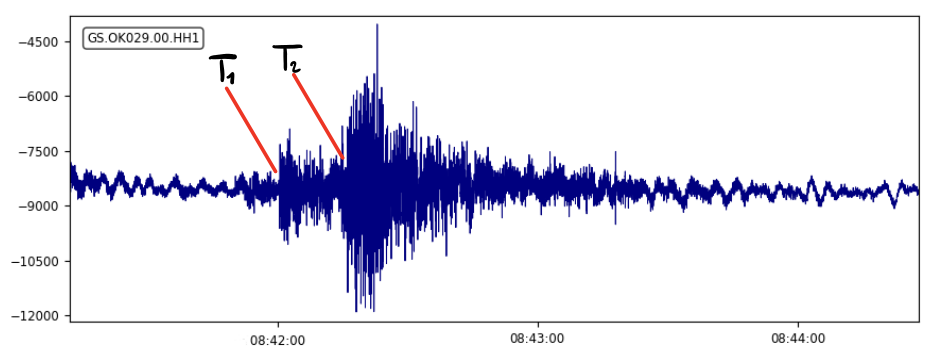
\includegraphics[width=\columnwidth]{../processed-data/problem-time-window-labeling.png}
  \caption{Illustration of the problem of tme window labeling}
	\label{fig:10min-example}
\end{figure}

\section{Feature Creation}

\section{Model Selection}

\section{Conclusion}

\section{Further improvements}

\begin{thebibliography}{9}
\bibitem{obspy}
ObsPy: python library to collect seismological data.
\\\texttt{https://docs.obspy.org/}
\end{thebibliography}

\end{document}
